\chapter{Neuromuscular Model}\label{sec:neuro_model}
\begin{marginfigure}
    \centering
    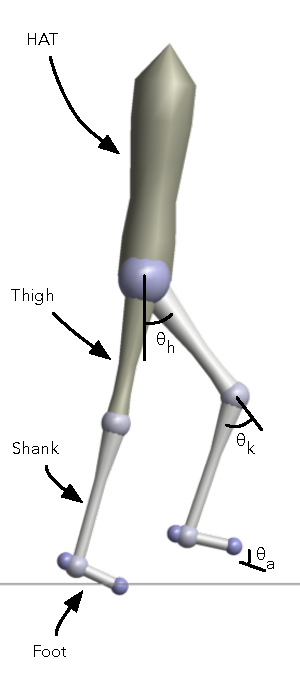
\includegraphics[width=\linewidth]{neuro_mech_model}
    \caption{The skeletal model we use to simulate neuromuscular reflex control.
    The model consists of seven segments: left and right feet, shanks, and
    thighs, as well as a lumped head-arms-trunk (HAT) segment. Flexion joint
    angles are positive, extension joint angles are negative, and the zero
    angle configuration represents standing.}
    \label{fig:neuro_seven_link}
\end{marginfigure}

In this thesis we intend to investigate the ability of neuromuscular reflex
control to improve amputee gait robustness. To this end, here we provide a more
detailed review the neuromuscular model components on which we base our
prosthesis control. Four parts comprise the model: a mechanical simulation
environment we use to obtain simulation results (\cref{sec:neuro_mech_model}),
biological motors modeled by the hill muscle model that apply torques to joints
(\cref{sec:neuro_hill_muscle}), and finally functionally-motivated stance
(\cref{sec:neuro_stance_reflexes}) and swing (\cref{sec:neuro_swing_reflexes})
reflexes that implement the key behaviors required for walking.

\section{Mechanical Model}\label{sec:neuro_mech_model}

To obtain the simulation results we present in this thesis, we construct a
mechanical model in the Matlab Simscape Multibody environment similar to those
presented in \citet{geyer2010muscle, song2015neural}. This model represents the
seven link biped in \cref{fig:neuro_seven_link} and includes two legs with
thigh, shank, and foot segments, as well as a lumped head-arms-trunk (HAT)
segment. \Cref{tab:model_mech_params} lists the segment lengths, center of mass
and joint locations measured from the distal end, masses, and inertias that
approximate those of a \unit[80]{kg}, \unit[2.0]{m} tall person.

\begin{table}[b]
  \centering
      \begin{tabular}{lllll}
        \toprule
        & Feet & Shanks & Thighs & HAT \\
        \midrule
        $l         \ (\unit{cm})$ & 20    & 50   & 50   & 80   \\
        $d_{COM}   \ (\unit{cm})$ & 14    & 30   & 30   & 35   \\
        $d_{Joint} \ (\unit{cm})$ & 16    & 50   & 50   &      \\
        $m         \ (\unit{kg})$ & 1.25  & 3.5  & 8.5  & 53.5 \\
        $J         \ (\unit{kg})$ & 0.005 & 0.05 & 0.15 & 3    \\
        \bottomrule
      \end{tabular}
  \caption{Segment lengths $(l_s)$, center of mass $(d_{COM})$ and joint
  $(d_{Joint})$ locations measured from the distal end, masses $(m)$, and
  inertias $(J)$ approximated from
  \citet{gunther2003synthesis}.}\label{tab:model_mech_params}
\end{table}

The mechanical model interacts with the environment through ground reaction
forces on the toes and balls of the feet. Specifically, we use a 2-dimensional
reduction of the 3D ground contact model presented in
\citet{song2013generalization} to calculate forces in the normal and
tangential directions with respect to the terrain. In the normal direction the
force is
\begin{align}
    F_n = k_n \Delta n_c (1 + \dot n_c) (\Delta n_c  > 0)
    \left(\nicefrac{\dot n_c}{v_{max}} > -1 \right),
    \label{eq:grf_n}
\end{align}
where $k_n = \unitfrac[78.45]{N}{mm}$ is the stiffness coefficient in
the normal direction and $\Delta n_c$ and $\dot n_c$ are the normal penetration
in the normal direction and velocity. The form of the normal force is inspired
by \citet{gunther2003synthesis, scott1993biomechanical} and represents a linear
spring with multiplicitive damping.  $v_{max} = \unitfrac[3]{cm}{s}$ represents
the maximum recovery velocity of the ground. If $\dot n_c$ exceeds this
velocity ground contact is lost.

In the tangential direction, a state machine switches between two force models
representing sliding and static frction. Static frction is given by
\begin{align}
    F_{t,sl} = -\func{sign}{\dot t_c} \mu_{sl} F_n
\end{align}
while static friction is given by
\begin{align}
    F_{t,st} = -k_t \Delta t_c \left(1 + \func{sign}{\Delta t_c}
    \frac{\dot t_c}{v_{max}} \right),
\end{align}
where $\Delta t_c$ is the penetration in the tangential direction $\dot t_c$
is the penetration velocity, $\mu_{sl} = 0.8$ is the sliding coefficient of
friction, and $k_t =\unitfrac[78.45]{N}{mm}$ is the stiffness coefficient in the
tangential direction.

Finally, the biped skeletal model includes soft joint limits to represent
the skeletal joint limits on the knee, ankle, and hip joints. The functional
form form the soft limit joint torque is identical to that of the normal ground
reaction force given by \cref{eq:grf_n}.
\begin{align}
    \tau_{jl} = k_{jl} \Delta \theta_{jl} (1 + \dot \theta_{jl}) (\Delta
    \theta_{jl}  > 0) \left(\nicefrac{\dot \theta_{jl}}{\dot \theta_{max}} > -1
    \right), 
    \label{eq:grf_n}
\end{align}
where $k_{jl} = \unitfrac[0.3]{N \cdot m}{deg}$ is the joint stiffness $\Delta
\theta$ and $\dot \theta_{jl}$ are the joint limit penetration angle and
velocity respectively, and $\dot \theta_{max} = \unitfrac[1]{deg}{s}$ is the
maximum joint limit retraction velocity. \Cref{tab:joint_lim} lists the
engagement angles for the joint limits.

\begin{margintable}
  \centering
      \begin{tabular}{lll}
        \toprule
        Joint & ext.\ lim.\ & flex lim.\ \\
        \midrule
        hip   & -40 & 50 \\
        knee  & 5 &      \\
        ankle & -40 & 20 \\
        \bottomrule
      \end{tabular}
  \caption{Joint limits for the hip, knee, and ankle joints listed in degrees.
  Positive joint angles represent flexion and negative joint angles represent
  extension (see \cref{fig:neuro_seven_link}).}\label{tab:joint_lim}
\end{margintable}

\section{Hill Muscle Models}\label{sec:neuro_hill_muscle}

\begin{marginfigure}
    \centering
    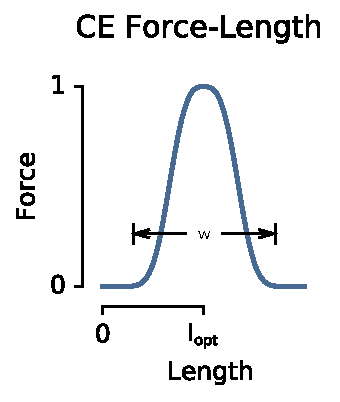
\includegraphics[width=\linewidth]{force_length_plot_annotate}
    \caption{}
    \label{fig:force_length_ce}
\end{marginfigure}

\begin{marginfigure}
    \centering
    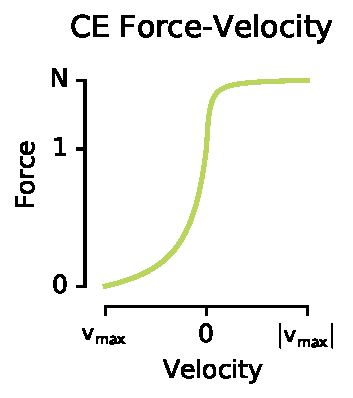
\includegraphics[width=\linewidth]{force_velocity_plot}
    \caption{}
    \label{fig:force_velocity_ce}
\end{marginfigure}

\begin{marginfigure}
    \centering
    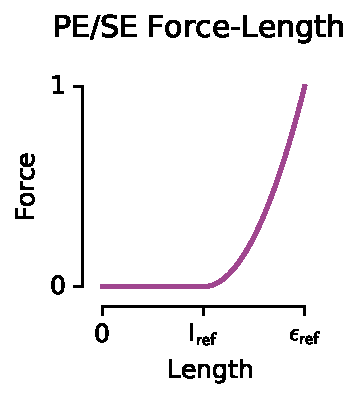
\includegraphics[width=\linewidth]{force_length_pese_plot}
    \caption{}
    \label{fig:force_length_pese}
\end{marginfigure}

\begin{margintable}
  \centering
  \begin{tabular}{ll|ll}
    \toprule
    Param & Value          & Param & Value      \\
    \midrule                        
    $\tau$ & \unit[0.1]{s} & $l_{opt}^{ham}$   & \unit[0.10]{m} \\
    $w$ & 0.56             & $v_{max}^{ham}$   & \unitfrac[-1.2]{m}{s} \\
    $K$ & 5                & $F_{max}^{ham}$   & \unit[3000]{N} \\
    $N$ & 1.5              & $l_{slack}^{ham}$ & \unit[0.31]{m} \\
    $\epsilon_{pe}$ & $w$  &                   &  \\
    $\epsilon_{se}$ & 0.04 &                   &  \\
    \bottomrule
  \end{tabular}
  \caption{Neuromuscular parameters for shared entities (left) and the hamstring
  muscle (right)}
  \label{tab:neurmusc_params}
\end{margintable}

\section{Stance Reflexes}\label{sec:neuro_stance_reflexes}
\section{Swing Leg Control}\label{sec:neuro_swing_reflexes}
\subsection{Idealized Swing Leg Control}
\subsection{Neuromuscular Reflex Swing Leg Control}
